% !TEX root = thesis.tex
\chapter{はじめに}
\label{chap:preface}
\section{ウェブ工学と機械学習}
近年ウェブ工学の領域においては、広告の効率アップや文章の分析、検索エンジンの性能向上などが求められている。このため、ユーザの性格や行動の分析、ネットワーク構造の未来予測、文章の意味や感情の理解といった技術が必要とされている。\par
例えば、ウェブ上で物を販売しているサイトにおいて、ユーザが購入しそうな商品を勧め、売り上げを増大させることを考える。ユーザが今まで見た商品、購入した商品を分析して、ユーザの求めている商品のジャンルを知ったり、ウェブショッピングにおける性格を知ることが出来れば、ユーザが買いたい商品を先回りして、広告表示することが出来る。ユーザに対して、より購入してくれそうな広告を多く見せて、広告の効率をアップさせることで、サイトからの収益が上がることが期待できる。\par
ウェブ工学では、ウェブ上のデータを元に知識を学習し、次に得た知識を用いて予測や分類を行う、というアルゴリズムが必要になっている。例えば、ユーザ行動やソーシャルネットワーク構造の傾向を学習して、将来の動向を予測したり、ユーザに送られたメールの意味を理解できるようになって、迷惑メールとそうでないものを分類できるようになる、といった具合である。こういった知識学習のためには、機械学習(Machine Learning)と呼ばれる手法が広く用いられている。\par
機械学習とは、対象となる知識を数学的なモデルで表し、より適切なモデルを求めて微修正を重ねることで、知識を洗練させていくアプローチである。使用する数学的なモデルの大筋は、経験を基にあらかじめ決めておく。ユーザ行動、リンク構造、メールの文章といった元データは、全て数値に変換されて、モデルに入力される。モデルは、入力データから予測や識別を実際に行いつつ、より良い結果が得られるように、モデル内の係数を調整していく。最終的に、多種多様なデータに対して、適切な予測や識別を行うことが出来る数学的モデルを得ることができるのである。

\section{深層学習の台頭}
機械学習における大きなポイントの1つに、元データをどのような数値データに変換するか、という問題がある。\par
機械学習の一般的なプロセスを、図\ref{c1_ml}に示す。変換された数値データのことを、 特徴量、あるいは素性(feature)と呼ぶ。機械学習は、「生データから素性への変換」「素性をモデルに入力」「モデルによる数値計算で、結果を出力」「結果がより正確になるよう、モデルを修正」というプロセスの繰り返しで成り立っている。このうち、「素性への変換」だけは、画像・文章・リンク構造といった、データの種類に依存している。いったん素性が数値の形で得られれば、残りのプロセスは、データの種類に依存せず、全て入力数値とモデルの関係だけで解決することができる。つまり、機械学習のプロセスは、データの種類に依存する素性変換と、汎用的に使えるモデル学習の部分に分かれているのである。
\begin{figure}[tbp]
 \centering
  
\includegraphics[width=80mm]{img/c1/ml}
 \caption{機械学習の一般的プロセス}
 \label{c1_ml}
\end{figure}
\par
機械学習の性能を上げるためには、素性への変換部分を工夫する方法と、使用する数学的モデルを洗練する方法の2つがある。素性への変換部分の改良は、対象となるデータの種類に強く依存している。例えば、画像データを素性数値に変換する場合、単純なRGB画素データをそのまま使っても良いが、SIFT特徴量\cite{lowe1999object}やSURF特徴量\cite{bay2008speeded}、フィッシャーベクトル\cite{perronnin2007fisher}など、より画像の特徴を捉えた特徴量を用いることが定石となっている。音声データに対しては、時間領域や周波数領域の波形をそのまま用いても良いが、メル周波数ケプストラム係数と呼ばれる特徴量も用いられる。問題とデータ種別に応じて、利用する特徴量を工夫することにより、機械学習の識別精度や実行時間などの性能が向上することが知られていた。このとき、特徴量はそれぞれのデータの専門家による、謂わば職人芸によって作られていた。\par
2000年代半ばに、深層学習と呼ばれる一群の手法が台頭した。深層学習とは機械学習の手法の1つで、人間の脳の構造に類似した、多層ニューラルネットワーク構造をモデルに用いて、学習を行わせる方法である。深層学習は、画像認識や音声認識、化合物の生成予測といった分野で優れた性能を示し、注目を浴びるようになった。図\ref{c1_nikkei}は、多層ニューラルネットワークが人間の脳の思考回路である、神経細胞のつながりを模倣する様子を表している。(日経ビジネス2013年4月号より一部抜粋)\\
\begin{figure}[tbp]
 \begin{center}
  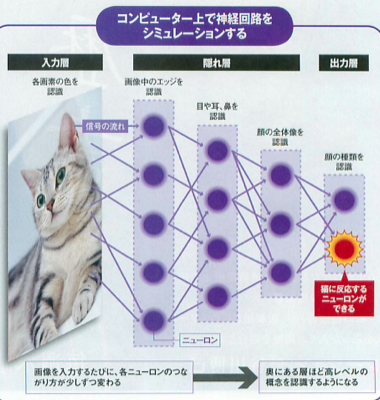
\includegraphics[width=80mm]{img/c1/nikkei}
 \end{center}
 \caption{深層学習で画像を認識する流れ}
 \label{c1_nikkei}
\end{figure}
深層学習の特徴の一つとして、生の入力データから自動的に素性を作り、抽象表現を習得する働きがあると考えられている。例えば人間の顔画像データを学習させた場合、多層ニューラルネットワークを構成する複数のレイヤーのうち、入力に近い低レイヤーのニューロンは、画像のエッジ部分に対して強く反応し、出力に近い高レイヤーのニューロンでは、目口鼻、さらに顔全体など、より抽象度の高い要素に対して反応することがわかった。これは、見方を変えれば、低レイヤーでは中間表現(素性にあたる)を抽出しており、低レイヤーで得た素性を高レイヤーに入力することにより、より高レベルな抽象的概念に対しても優れた識別精度を実現している、と考えられる。どのような素性を使えば良い結果が出るのか、素性の抽出方法自体を同時に機械学習していることから、深層学習は表現学習(表現学習)とも呼ばれている。\par
図\ref{c1_lee2009_faces}は、2009年、Leeらによる深層畳み込み信念ネットワークの実験によって学習された顔の要素である。上が2レイヤー目、下が3レイヤー目で、2レイヤー目では、鼻や口、目といった顔を構成するパーツが学習されている。これは、単なる画素の数値に比べて、明らかに抽象度の高い情報に反応していると言える。さらに、3レイヤー目では人間の顔を学習することに成功している。2レイヤー目で作り出した、「顔のパーツ」という素性を元にして、さらに抽象度の高い、人間の顔という要素を推論しているのである。\cite{lee2009convolutional}
\begin{figure}[tbp]
 \centering
  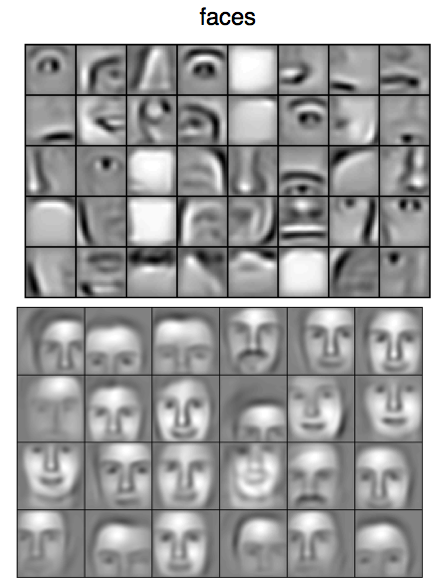
\includegraphics[width=80mm]{img/c1/lee2009_faces}
 \caption{深層学習による、顔の構成要素の学習結果}
 \label{c1_lee2009_faces}
\end{figure}
\par

Googleの深層学習研究グループは2012年、Youtubeのビデオから抽出した静止画による教師無し学習によって、人間や猫の顔画像を識別できる多層ニューラルネットワークモデルの学習に成功し、大きな話題を呼んだ\cite{le2012building}(それぞれ\ref{c1_facedetection}と\ref{c1_catdetection}、Googleの研究紹介記事\footnote{\url{http://googleblog.blogspot.jp/2012/06/using-large-scale-brain-simulations-for.html}})と論文\cite{le2012building}より引用)。\par
\begin{figure}[tbp]
 \begin{center}
  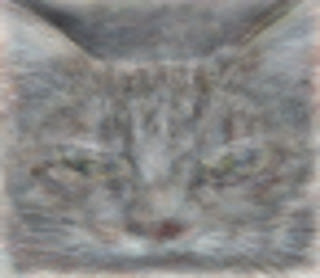
\includegraphics[width=50mm]{img/c1/cat_detection}
 \end{center}
 \caption{猫を認識するニューロン (教師無しYoutubeビデオより学習された。)}
 \label{c1_catdetection}
\end{figure}

\begin{figure}[tbp]
 \begin{center}
  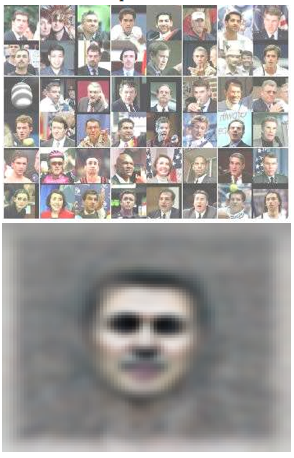
\includegraphics[width=50mm]{img/c1/google_face}
 \end{center}
 \caption{上 : 入力画像の中で、ニューロンが最も強く反応した48枚 下 : 計算上、最もニューロンが強く反応する画像}
 \label{c1_facedetection}
\end{figure}


\section{深層学習の課題と、研究の目的}
深層学習が高い識別性能を持つことがわかり、深層学習を身近な問題に適用して、良い成果を得たいという機運が高まっている。例えば、ウェブ工学の分野では機械学習が大きな役割を果たしており、この学習プロセスに深層学習を組みこむことで、学習精度が向上したり、より多様な情報を扱えるようになる可能性がある。出来るだけ簡易に、深層学習を様々な問題に応用するための方法論が求められている。\par
しかし、深層学習は歴史の浅い発展途上の技術であり、どのアルゴリズムを定番とすれば良いのか、試行錯誤の段階にある。これは、各アルゴリズムの改良点が次々と見つかっていることに加え、学習性能が高くなる原理や、各アルゴリズムの得手不得手など、解明されていない部分が多いことが、主な原因である。アルゴリズムが開発途上で確定できていないため、公開されているライブラリも、現状では、開発用途や実験的なものが多くなってしまっている。実験的なライブラリでは、一部の種類のデータにのみ適用されることを想定して書いている場合があり、他の種類のデータを扱うためには、データ変換用のソースコードを記述しなければならないケースが多い。そもそも有力なアルゴリズムに対応する実装が公開されていない場合もあり、この場合、アルゴリズムの部分も含めて全ての実装を用意しなければならない。また、問題に応じて自らアルゴリズムの細部を調整しなければならない場合もある。例えば、学習の繰り返し回数(エポック数)や、どの種類のレイヤーを何回重ねるべきか(レイヤー構造)、1つのレイヤーに含まれる学習素子(ニューロン)の個数はどうするか、などである。これらはソースコードの作成者が経験的に手作業で調整しているケースが多く、標準と言える公開ライブラリが確立していない状況なので、ウェブ工学など応用分野に深層学習を適用したいと考えても、プログラム開発に長い時間がかかってしまう。開発における大きな障壁となっている。\par
さらに、現在の深層学習技術では、他のアルゴリズムに比べて学習にかかる時間が長いことが多く、ハードウェア性能が低いマシンでは、アルゴリズムを実用的な時間で実行すること自体が容易ではない。例えば、先述したGoogleの研究では、1000台のマシンによるクラスタを用いても、訓練に3日間かかっており、個人レベルでは実験自体がほぼ不可能である\cite{le2012building}。必要実行時間の長さをカバーするため、GPUを用いて演算をスピードアップさせる手法が確立されつつあるが、特殊なプログラミングが要求され、開発における障壁の1つとなっている。また、ノートパソコンの大部分など、並列演算に利用可能なGPUを搭載していないパソコンを使っている場合には、ライブラリがGPUを利用しているために、却ってその実行が不可能になってしまうこともある。(これは4章にて詳しく述べる。)\par
手元のパソコンにて実行可能な深層学習のソースを探し当てたとしても、このソースが実際に、論文にて示されているような高い精度を実現できるかどうかは、定かではない。深層学習の分野では、実験に用いたソースコードが提供されている場合もいくつかあるが、単にアルゴリズムの要点を示すためのものだったり、ハイパーパラメータが実行時間の短縮を重視した、言わばお試し用の状態になっていて、論文に記述してある精度を手元のパソコンで実現することが難しい場合がある。\par
以上に挙げた原因により、深層学習技術に関心を持っていても、まず実際の問題に深層学習を試行すること自体が困難であり、応用技術開発のハードルは更に高くなっている。特に、国内での研究開発は遅れており、早急なキャッチアップが必要である。\par
本研究では、このような現状を踏まえ、深層学習技術をウェブ工学など実際の問題に応用するために、「分類精度の再現が難しい」「学習時間が長く、速度上昇のためのGPU使用もハードルを上げている」「ライブラリが未成熟なため、応用や改良が難しい」という上で挙げた実装における問題点を、出来る限り緩和することを目指す。\par
2章では、従来のウェブ工学における機械学習の応用方法と、深層学習出現以前に良く用いられていた、機械学習による識別器学習方法について、俯瞰する。3章では、深層学習を構成する個々のアルゴリズムについて、その原理と詳細を述べる。4章では、実際に深層学習アルゴリズムを利用する上で、どのように実装を進めれば、先に上げた問題点を緩和できるのかを述べる。5章では、深層学習のプログラムを、汎用的なベンチマークにかけることで、その性能を測定・比較する。6章では、5章までの結果を受けて、深層学習を利用していく上でのベストプラクティスを考察する。
%7章では、深層学習の利用例として、ソーシャルネットワークにおけるプロフィール推定を行う。
